\documentclass[a4paper]{article}

%deixa no padr?o brasileiro, traduzindo as se??es, possibilitando caracteres e hifen
\usepackage[brazilian]{babel}
\usepackage[utf8]{inputenc}
\usepackage[T1]{fontenc}
\usepackage{amsmath,amsthm,array} 

%estilo de header
\pagestyle{headings}

%pacote para inserir imagem
\usepackage{graphicx}

%t?tulo
\title{Redes Auto-Organizáveis: Mapas de Kohonen}
\author{Gustavo Scaloni Vendramini    \\ 
        Guilherme José Henrique       \\
        Sean Carlisto de Alvarenga    \\
        Vinícius Fernandes de Jesus}
\date{\today}

%pacote que coloca links no table of contents e monta o índice lateral, de acordo com as se??es do documento.
\usepackage[pdftex]{hyperref}

\begin{document}
\maketitle

\begin{abstract}
Este artigo apresenta uma implementação de um modelo de rede neural auto-organizável conhecida como mapas auto-organizáveis de Kohonen ou redes SOM (do inglês \textit{Self-Organizing Maps}).
\end{abstract}

\section{Redes SOM}\label{som}
Mapas auto-organizáveis ou Mapas de Kohonen são um tipo de rede neural. Foram desenvolvidos em 1982 por Tuevo
Kohonen, professor emérito da Academia da Finlândia. SelfOrganizing mapas são apropriadamente chamado. "Auto-organização" é porque a supervisão não é
necessária. SOMs aprendem por conta própria através da aprendizagem competitiva não supervisionada.
"Mapas" significa que eles tentam mapear seus pesos para entrar em conformidade com os determinados
dados de entrada. Os nós de uma rede SOM tentam tornar-se igual às entradas 
que lhes são apresentados. Neste sentido, é assim que eles aprendem. Especificamente, o relacionamento topológico das entradas de entrados topológicos
são conservados quando mapeado para uma rede SOM. Isso tem um valor sensato
para a representação de dados complexos.

\subsection{Estrutura}

A Figura \ref{som-node} é uma rede SOM 4x4 (4 nós para baixo, quatro nós de diâmetro). 
cada mapa está ligado a cada nó de entrada. Para este pequeno nó 4x4
de rede, resulta em 4x4x3 = 48 ligações. Em segundo lugar, perceber que nós do mapa não são
ligados uns aos outros. Os nós são organizados desta maneira, como uma grade de duas dimensões
faz com que seja fácil de visualizar os resultados. Esta representação é também útil quando o
Algoritmo SOM é usado. Nesta configuração, cada nó tem um única coordenada (i, j).
Isto torna mais fácil de fazer referência a um nó na rede, e
calcular as distâncias entre os nós. Devido às ligações apenas para o
nós de entrada, os nós mapa são indiferentes quanto ao valor que os seus vizinhos têm.
Um nó de mapa só vai atualizar seus pesos "(explicado a seguir), com base no que o vetor de entrada
fornece de informação.

\begin{figure}[ht]
\centering
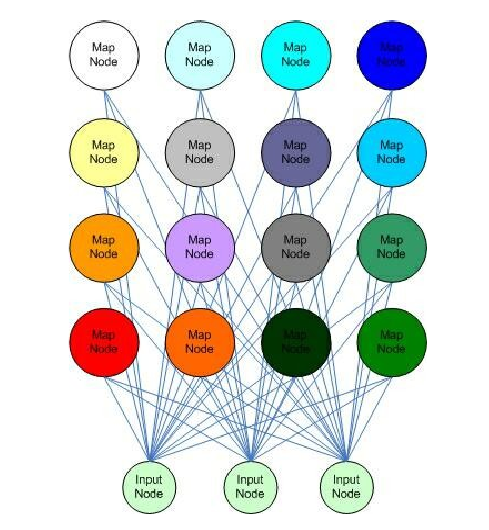
\includegraphics[width=1\textwidth]{imgs/node-som.png}
\caption{Nó do Mapa de Kohonen}
\label{fig:som-node}
\end{figure}

\subsection{Treinamento}\label{treinamento}
A rede SOM utiliza um algoritmo de aprendizado competitivo e não-supervisionado. Um padrão de entrada é apresentado a rede, um neurônio vence e inicia a atualização de seus pesos e de seus vizinhos (até um raio de vizinhança). Isto repete para cada nova entrada e a taxa de aprendizado e o raio de vizinhança são decrementados durante o processo \cite{Braga,Haykin}. A atualização dos pesos do neurônio vencedor e de seus vizinhos é dada como segue:

\[ w_{ji}(t+1) = \left\{ 
  \begin{array}{l l}
    w_{ji}(t) + \eta(t)(x_{i}- w_{ji}(t)) & \quad \text{se j $\in$ $\Lambda$(t)}\\
    w_{ji}(t) & \quad \text{caso contrário}
  \end{array} \right.\]

Onde $w_{ji}$ é o peso entre os neurônios i e j, $\eta(t)$ é a taxa de aprendizado e $\Lambda$ é a vizinhança.

\begin{verbatim}
1:  Inicializar pesos e parâmetros;
2:  repita
3:     para todo padrão de treinamento faça
4:        Definir neurônio vencedor;
5:        Atualizar os pesos deste neurônio e de seus vizinhos;
6:        se o número do ciclo for múltiplo de N então
7:           Então reduzir a taxa de aprendizado;
8:        fim-se
9:     fim-para
10: até que mapa de características não mudar
\end{verbatim}

\subsection{Classificação de Cor}
Este é considerado o ``Hello World'' de SOMs. A maioria dos tutoriais publicados no
SOMs usam a classificação de cor como seu principal exemplo. Isto é para uma boa razão. Ao passar por este exemplo, o conceito de SOMs pode ser solidamente apreendido. A razão pela qual a classificação de cor é bastante fácil de entender é por causa da quantidade relativamente pequena de dados utilizados, bem como o aspecto visual dos dados.

A classificação de cores do SOM usam apenas três pesos por nó de saída e nós de entrada. Estes pesos representam a tripla (r, g, b) para a cor. Por exemplo, as cores podem ser apresentado à rede, (1,0,0) para o vermelho, (0,1,0) para o verde, etc. A meta para a rede aqui é aprender a representar todas essas cores de entrada em sua grade de duas dimensões. Com isso em mente, se azul escuro e azul claro são apresentados ao SOM, eles devem acabar ao lado do outro na grade de rede.

Para ilustrar o processo passo a passo do algoritmo de classificação da cor, o primeiro passo consiste em inicializar a rede, como mostra a figura \ref{fig:initial-node}.

\begin{figure}[ht]
\centering
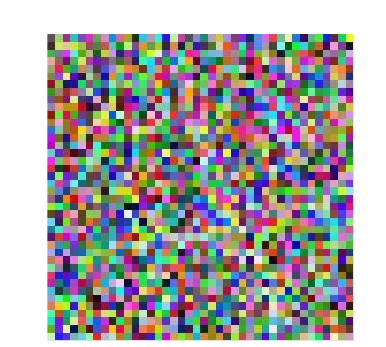
\includegraphics[width=0.7\textwidth]{imgs/initial-node.png}
\caption{Disposição inicial dos neurônios}
\label{fig:initial-node}
\end{figure}


Em seguida, temos que escolher um vetor de forma aleatória a partir dos vetores de entrada. Oito vetores de entrada são utilizados neste exemplo, que vão do vermelho para o amarelo para verde escuro. 

Posteriormente, o próximo passo é passar por cada nó e encontrar BMU (Best Matching Unit, utilizando a distância euclidiana, por exemplo). A Figura \ref{fig:bmu-node} mostra o BMU sendo selecionado na rede 4x4.

Com o BMU encontrada, o raio vizinhança deve ser calculado, como também mostrado na Figura \ref{fig:bmu-node}. Todos os nós em vermelho estão dentro do raio. 

Por último, aplica-se o aprendizado para todos esses nós. O aprendizado baseia-se na distância do neurônio em relação a entrada apresentada.

\begin{figure}[ht]
\centering
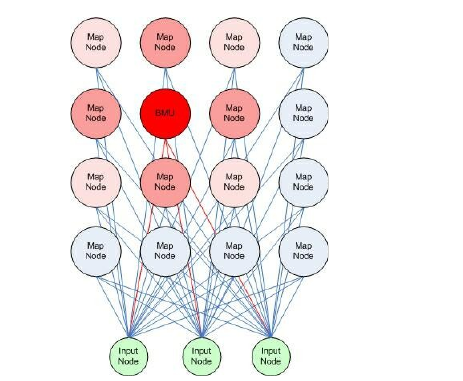
\includegraphics[width=0.7\textwidth]{imgs/node-bmu.png}
\caption{Nó vencedor}
\label{fig:bmu-node}
\end{figure}

Em seguida, um novo vetor aleatório é escolhido e todo processo se repete. A Figura \ref{fig:final-node} mostra um SOM treinado, representando todas as cores das oito entradas de cores. Observe como a cor verde fica ao lado do verde escuro e a cor vermelha está ao lado da cor laranja.

\begin{figure}[ht]
\centering
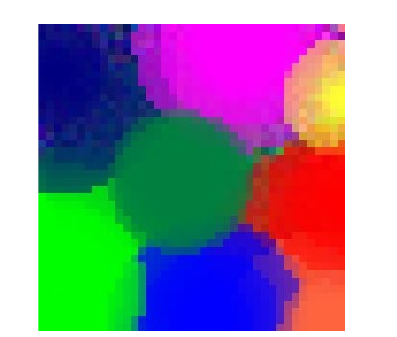
\includegraphics[width=0.5\textwidth]{imgs/final-node.png}
\caption{Estrutura do nó final}
\label{fig:final-node}
\end{figure}

%!TEX root = ../artigo.tex
\section{Resultados}
A rede neural auto-organizável implementada nesse trabalho, utilizou o algoritmo Mapa de Kohonen, desenvolvido por
Teuvo Kohonen em 1982 \cite{Kohonen}. A implementação deste trabalho pode ser vista em \url{https://github.com/QSF/ia-kohonen}.

Para os resultados práticos, a rede foi treinada com um conjunto de 1728 exemplos de dados reais, fornecidos pelo site \textit{UCI Machine Learning Repository}\footnote{http://archive.ics.uci.edu/ml/}, variando valores da taxa de aprendizado, pesos iniciais, raio da vizinhança e quantidade de neurônios na rede. O conjunto de exemplos escolhido foi o \textit{Car Evaluation}\footnote{http://archive.ics.uci.edu/ml/datasets/Car+Evaluation}, onde dados os atributos preço de compra do veículo, custo da manutenção, quantidade de portas do veículo, número de passageiros, tamanho do bagageiro e segurança estimada do veículo, avalia se o veículo é aceitável, inaceitável, bom ou muito bom.

Uma vez que o algoritmo Mapa de Kohonen organiza ou agrupa dimensionalmente os dados, o conjunto de exemplos foi adaptado, apresentando somente três dimensões (preço de compra do veículo, custo da manutenção e segurança estimada do veículo). O primeiro e segundo atributo aceitos os valores {low, med, high e vhigh}, enquanto que o útilo aceita os valores {low, med, high}.

Com o conjunto de dados coletados, algumas entradas foram testadas para verificar a modificação final da rede. Esses testes serão exibidos a seguir, sendo dividido pela quantidade de neurônios na camada de saída (16, 20, 25 e 36 neurônios).

\subsection{16 neurônios} % (fold)
\label{sub:16_neuronios}

\begin{figure}[ht!]
	\centering
	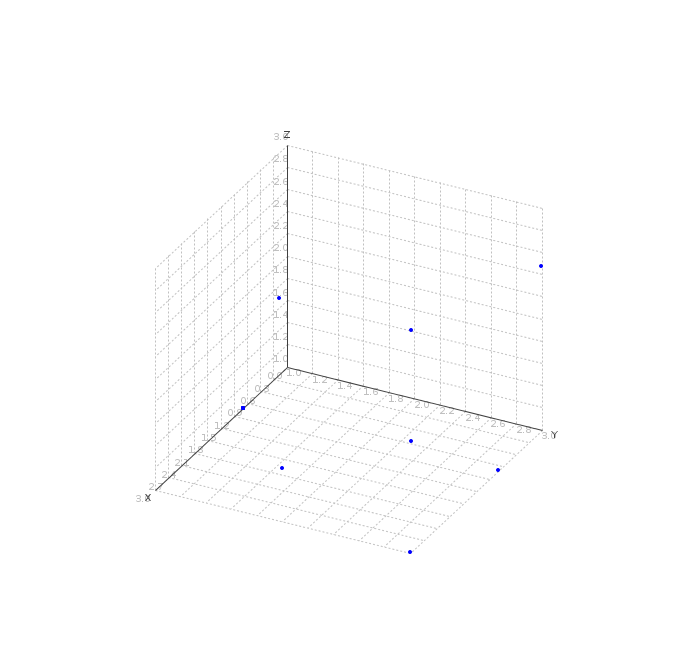
\includegraphics[scale=0.4]{./imgs/fig:out_16_teste_1}
	\caption{16 Neurônios - Teste 1}
	\label{fig:out_16_teste_1}
\end{figure}

\begin{figure}[ht!]
	\centering
	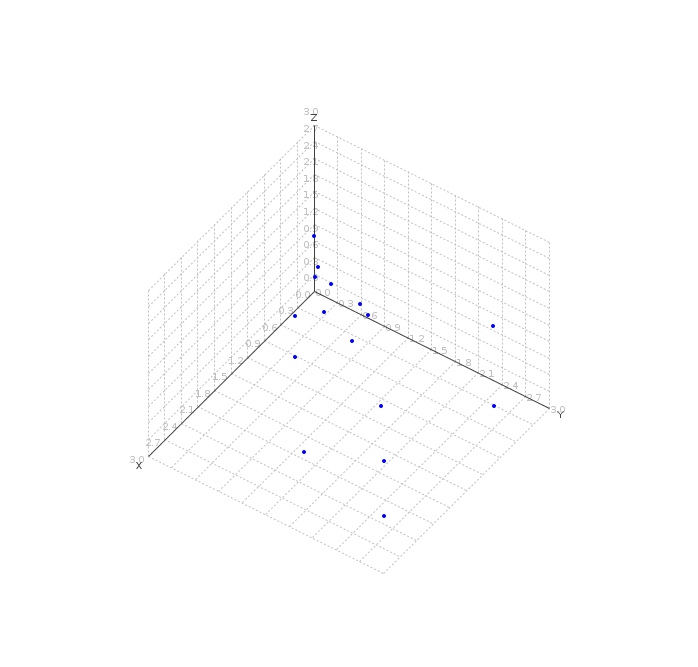
\includegraphics[scale=0.4]{./imgs/fig:out_16_teste_2}
	\caption{16 Neurônios - Teste 2}
	\label{fig:out_16_teste_2}
\end{figure}

\begin{figure}[ht!]
	\centering
	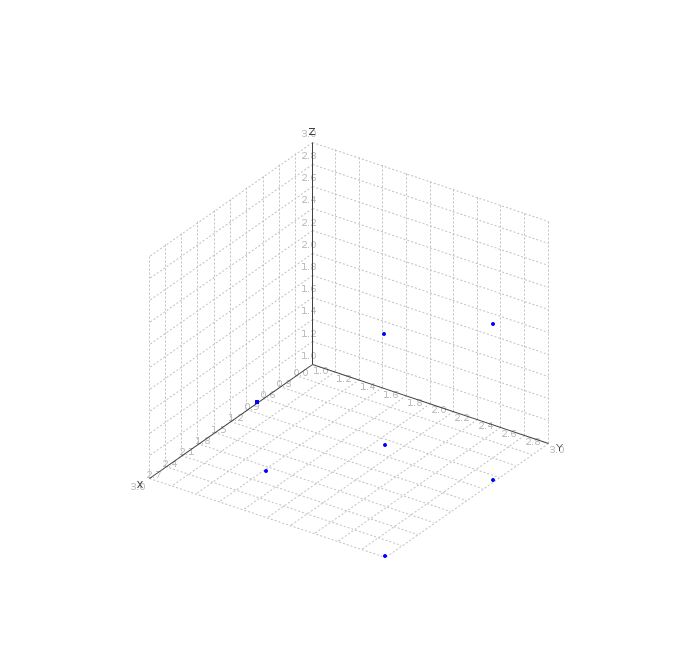
\includegraphics[scale=0.4]{./imgs/fig:out_16_teste_3}
	\caption{16 Neurônios - Teste 3}
	\label{fig:out_16_teste_3}
\end{figure}

\begin{figure}[ht!]
	\centering
	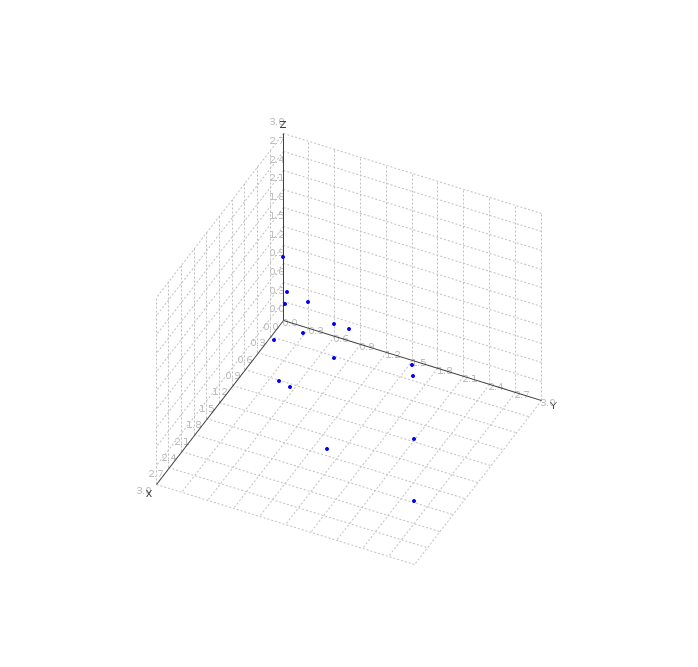
\includegraphics[scale=0.4]{./imgs/fig:out_16_teste_4}
	\caption{16 Neurônios - Teste 4}
	\label{fig:out_16_teste_4}
\end{figure}

Nos conjuntos de teste apresentados por essa seção, a rede possuia 16 neurônios na camada de saída, sendo que sua topologia é da forma de uma grade 4x4.

Para realizar os testes na rede mencionada, foi variado o valor da taxa de aprendizagem e dos pesos inicias, com raio fixo em 0.

Quatro testes foram executados, onde a configuração da rede para cada caso é ilustrada em ~\ref{table:dados_16}.
\begin{table}[ht]
\caption{Configurações da Rede com 16 Neurônios na Saída}
\centering
\begin{tabular}{|c|c|c|}  \hline
   Teste 	& Taxa de Aprendizagem 	& Pesos Inicias 	\\ \hline
   1 		& 0.1 				 	& todos 1 			\\ \hline
   2 		& 0.1 				 	& Random 			\\ \hline
   3 		& 0.3 				 	& todos 1 			\\ \hline
   4 		& 0.3 				 	& Random 			\\ \hline
\end{tabular}
\label{table:dados_16}
\end{table}

As figuras \ref{fig:out_16_teste_1}, \ref{fig:out_16_teste_2}, \ref{fig:out_16_teste_3} e \ref{fig:out_16_teste_4} representam a rede após a execução dos testes 1, 2, 3 e 4; respectivamente.

% subsection 16_neuronios (end)

\subsection{20 neurônios} % (fold)
\label{sub:20_neuronios}

\begin{figure}[ht!]
	\centering
	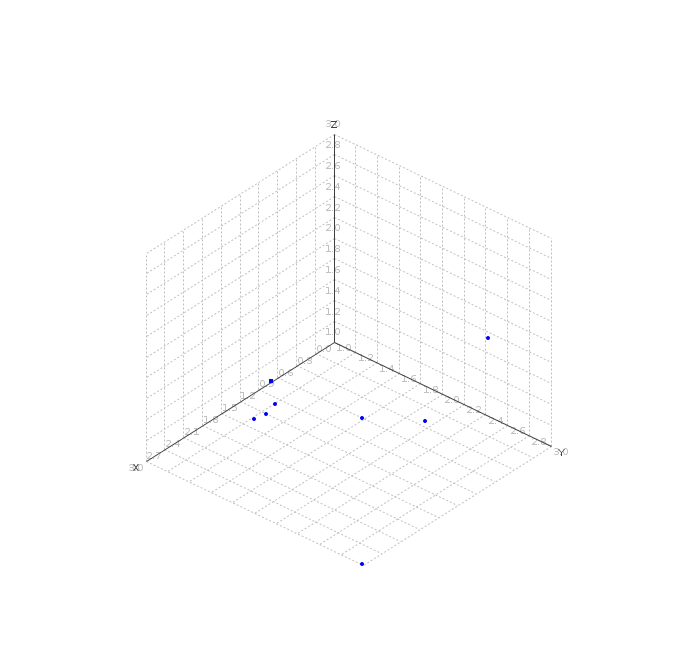
\includegraphics[scale=0.4]{./imgs/fig:out_20_teste_1}
	\caption{20 Neurônios - Teste 1}
	\label{fig:out_20_teste_1}
\end{figure}

\begin{figure}[ht!]
	\centering
	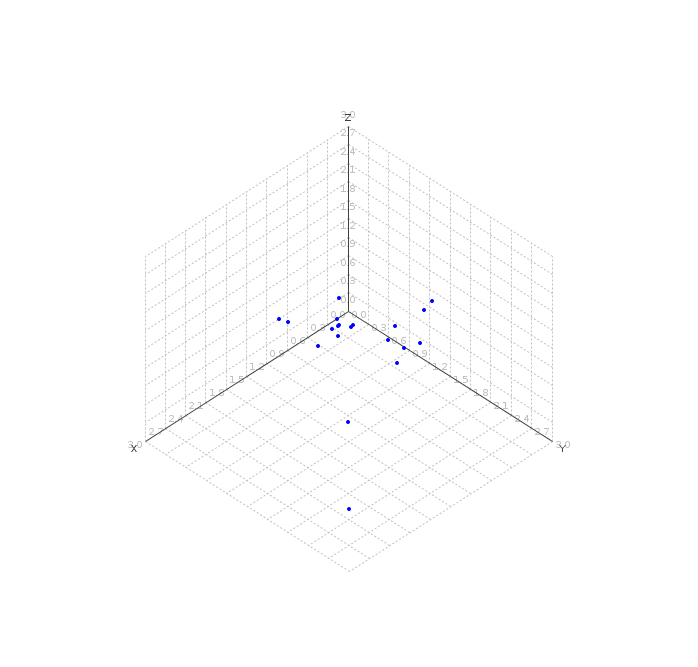
\includegraphics[scale=0.4]{./imgs/fig:out_20_teste_2}
	\caption{20 Neurônios - Teste 2}
	\label{fig:out_20_teste_2}
\end{figure}

\begin{figure}[ht!]
	\centering
	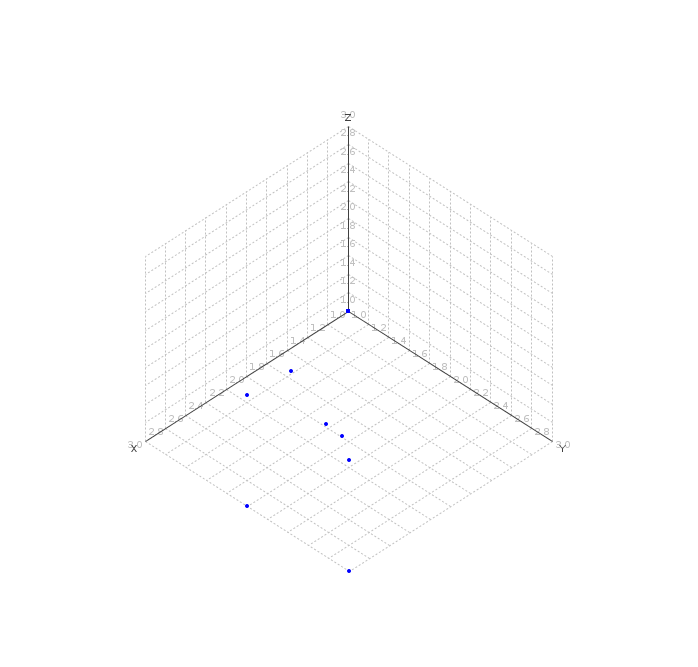
\includegraphics[scale=0.4]{./imgs/fig:out_20_teste_3}
	\caption{20 Neurônios - Teste 3}
	\label{fig:out_20_teste_3}
\end{figure}

\begin{figure}[ht!]
	\centering
	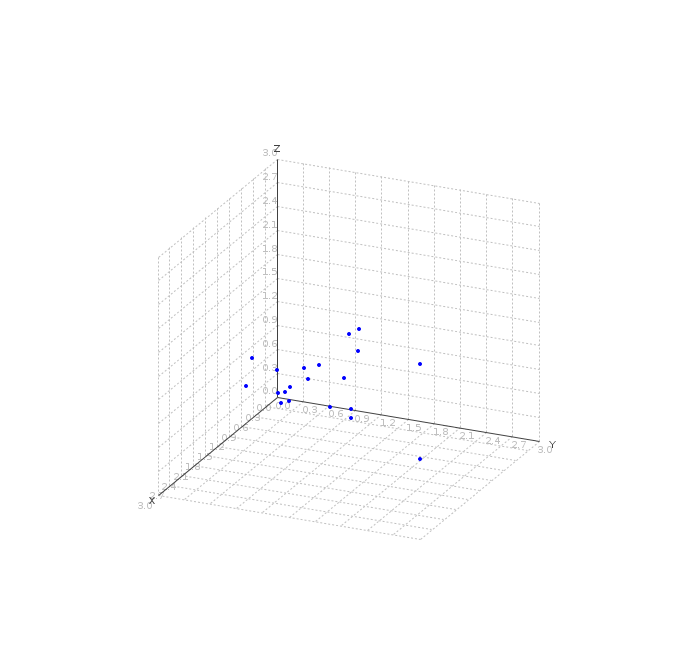
\includegraphics[scale=0.4]{./imgs/fig:out_20_teste_4}
	\caption{20 Neurônios - Teste 4}
	\label{fig:out_20_teste_4}
\end{figure}

Nesta seção, a rede possuia 20 neurônios na camada de saída, sendo uma grade 4x5.

Para realizar os testes na rede mencionada, novamente foi variado o valor da taxa de aprendizagem e dos pesos inicias, mas com raio fixo em 1.

Também foram executados quatro testes que tem sua configuração ilustrada na tabela ~\ref{table:dados_20}.
\begin{table}[ht]
\caption{Configurações da Rede com 20 Neurônios na Saída}
\centering
\begin{tabular}{|c|c|c|}  \hline
   Teste 	& Taxa de Aprendizagem 	& Pesos Inicias 	\\ \hline
   1 		& 0.5 				 	& todos 1 			\\ \hline
   2 		& 0.5				 	& Random 			\\ \hline
   3 		& 0.75 				 	& todos 1 			\\ \hline
   4 		& 0.75				 	& Random 			\\ \hline
\end{tabular}
\label{table:dados_20}
\end{table}

Os testes 1, 2, 3 e 4 são representados pelas imagens \ref{fig:out_20_teste_1}, \ref{fig:out_20_teste_2}, \ref{fig:out_20_teste_3} e \ref{fig:out_20_teste_4}; respectivamente.

% subsection 20_neuronios (end)

\subsection{25 neurônios}
Os gráficos a seguir mostram a plotação dos pontos após a execução do algoritmo para alguns valores de parâmetros e para 
uma rede com 25 neurônios. Apesar de não se poder afirmar se o algoritmo convergiu, vemos que aumentando o raio de vizinhança,
o algoritmo consegue ``especializar'' melhor o conjunto. O efeito da taxa de aprendizado está sobre a velocidade na qual o 
algoritmo irá convergir. Ela geralmente é dada empiricamente, assim como os pesos iniciais, que segundo \cite{Kohonen}, se forem
inicializados com valores iguais, faz o algoritmo convergir mais rapidamente.

\begin{figure}[ht!]
	\centering
	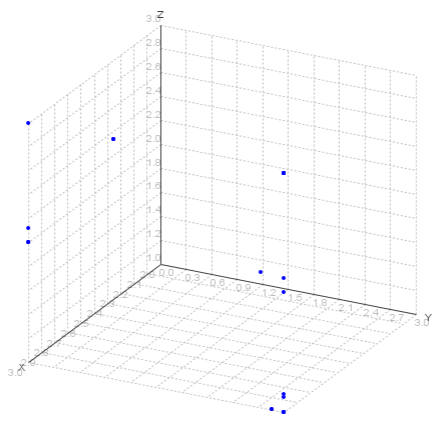
\includegraphics[scale=0.65]{./imgs/2a1.png}
	\caption{Taxa de aprendizado: 0.8662815917277779; Raio: 1; Pesos iniciais: A}
\end{figure}

\begin{figure}[ht!]
	\centering
	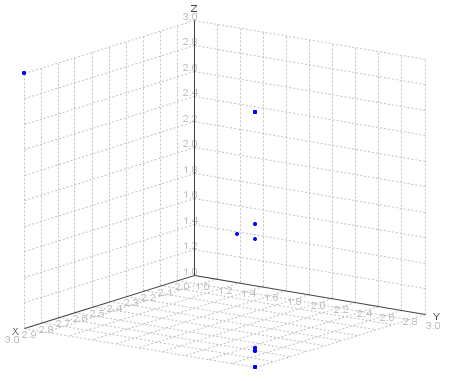
\includegraphics[scale=0.65]{./imgs/2a2.png}
	\caption{Taxa de aprendizado: 0.8662815917277779; Raio: 2; Pesos iniciais: A}
\end{figure}

\begin{figure}[ht!]
	\centering
	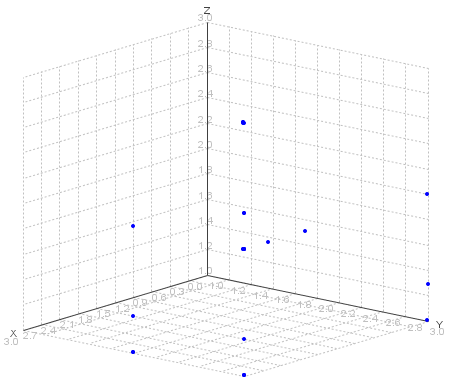
\includegraphics[scale=0.65]{./imgs/2b1.png}
	\caption{Taxa de aprendizado: 0.5980629675758204; Raio: 1; Pesos iniciais: B}
\end{figure}

\begin{figure}[ht!]
	\centering
	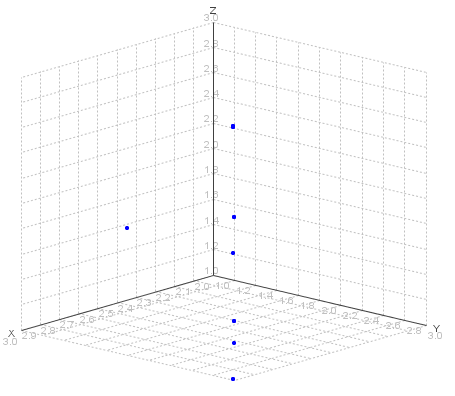
\includegraphics[scale=0.65]{./imgs/2b2.png}
	\caption{Taxa de aprendizado: 0.5980629675758204; Raio: 2; Pesos iniciais: B}
\end{figure}

\subsection{36 neurônios}
Os gráficos a seguir mostram a plotação dos pontos após a execução do algoritmo para alguns valores de parâmetros e para
uma rede com 36 neurônios.

\begin{figure}[ht!]
	\centering
	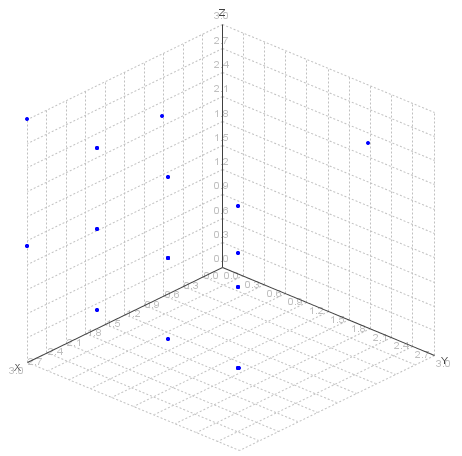
\includegraphics[scale=0.65]{./imgs/2d1.png}
	\caption{Taxa de aprendizado: 0.2625656059885696; Raio: 1; Pesos iniciais: D}
\end{figure}

\begin{figure}[ht!]
	\centering
	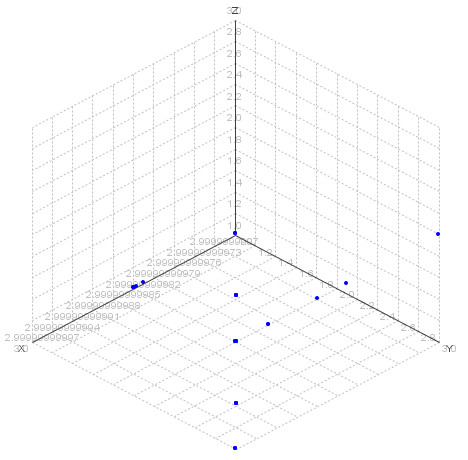
\includegraphics[scale=0.65]{./imgs/2d2.png}
	\caption{Taxa de aprendizado: 0.2625656059885696; Raio: 2; Pesos iniciais: D}
\end{figure}

\begin{figure}[ht!]
	\centering
	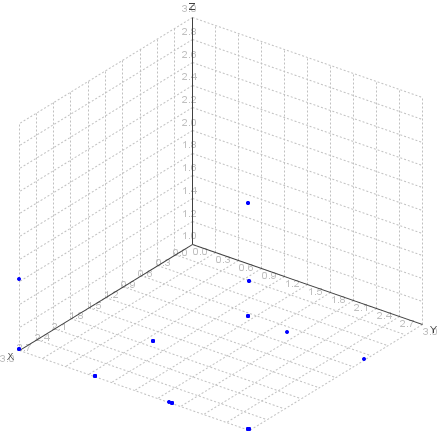
\includegraphics[scale=0.65]{./imgs/2e1.png}
	\caption{Taxa de aprendizado: 0.5517820314689292; Raio: 1; Pesos iniciais: E}
\end{figure}

\newpage
\begin{figure}[ht!]
	\centering
	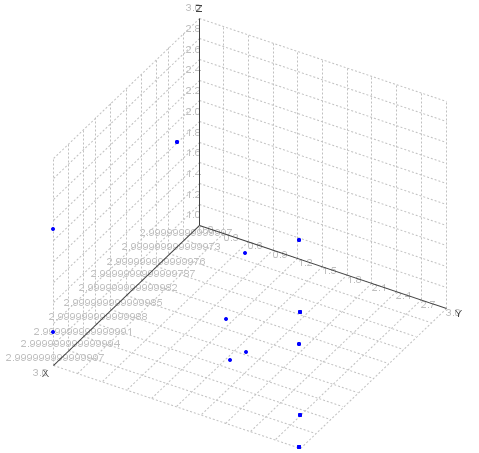
\includegraphics[scale=0.65]{./imgs/2e2.png}
	\caption{Taxa de aprendizado: 0.5517820314689292; Raio: 2; Pesos iniciais: E}
\end{figure}



\bibliographystyle{plain}
\bibliography{artigo}

\end{document}